\chapter{Neurons, Action Potentials and Synapses}\label{ch:b2:neurons-synapses}

Tap the tendon below the kneecap and the leg kicks, thirty
milliseconds later. In that time a stretch has been sensed in the
thigh, a signal has travelled a metre to the spinal cord, crossed
one junction to a second cell, travelled a metre back and set a
muscle contracting --- the whole round trip faster than a blink. No
\omterm{def:b2:cell-signalling:kinds}{hormone} could do this; it is done by cells built to conduct, and by
a signal that is not a substance moving but a wave of electricity
regenerated along a membrane. This chapter is about that cell and
that signal: the voltage a \omterm{def:b2:neurons-synapses:neuron}{neuron} keeps across its membrane, the
impulse it fires and how the impulse travels, and the \omterm{def:b2:neurons-synapses:synapse}{synapse} where
the electrical signal is turned into a chemical one and back again.

\section{The neuron}

\begin{definition}[Neuron, axon, nerve]\label{def:b2:neurons-synapses:neuron}
\index{neuron}\index{axon}\index{dendrite}\index{myelin}\index{glia}
A \emph{neuron} is a cell specialised for signalling: a cell body
(\emph{soma}) with the nucleus, branching \emph{dendrites} that
receive signals, and a single \emph{axon} --- a cable from a
micrometre to twenty micrometres thick and up to a metre long ---
that carries its output to \emph{terminals} on other cells. The
human brain has some $10^{11}$ neurons and each makes about a
thousand \omterm{def:b2:neurons-synapses:synapse}{synapses}. Neurons are outnumbered by \emph{glia}: astrocytes
that feed and buffer them, microglia that police them, and the
cells that wrap axons in \emph{myelin} --- dozens of turns of their
own membrane, nearly free of cytoplasm, forming an insulating sheath
interrupted every millimetre or so at the \emph{nodes of Ranvier}.
A \emph{nerve} is a bundle of thousands of axons, sensory and motor,
running together in connective tissue. Neurons do not divide in the
adult (with few exceptions), and an axon cut from its body dies; a
neuron is a cell that must last a lifetime.
\end{definition}

\begin{omfigure}
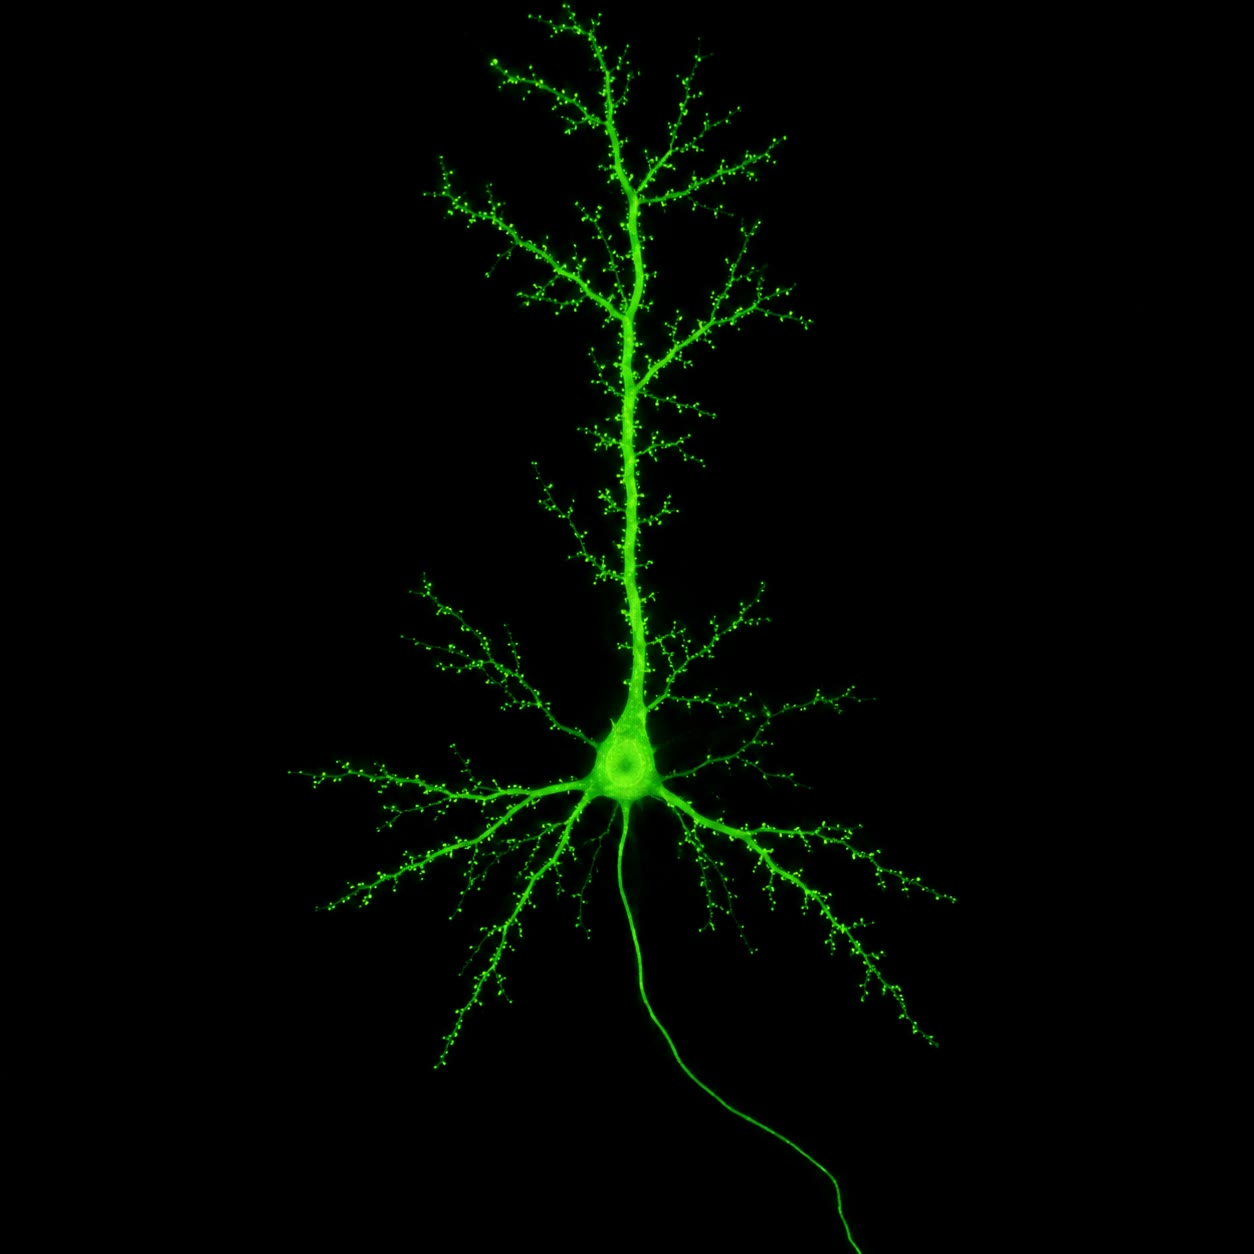
\includegraphics[width=0.4\linewidth]{images/book4/ai/b4-20-neuron-fluorescence.jpg}\hspace{0.05\linewidth}
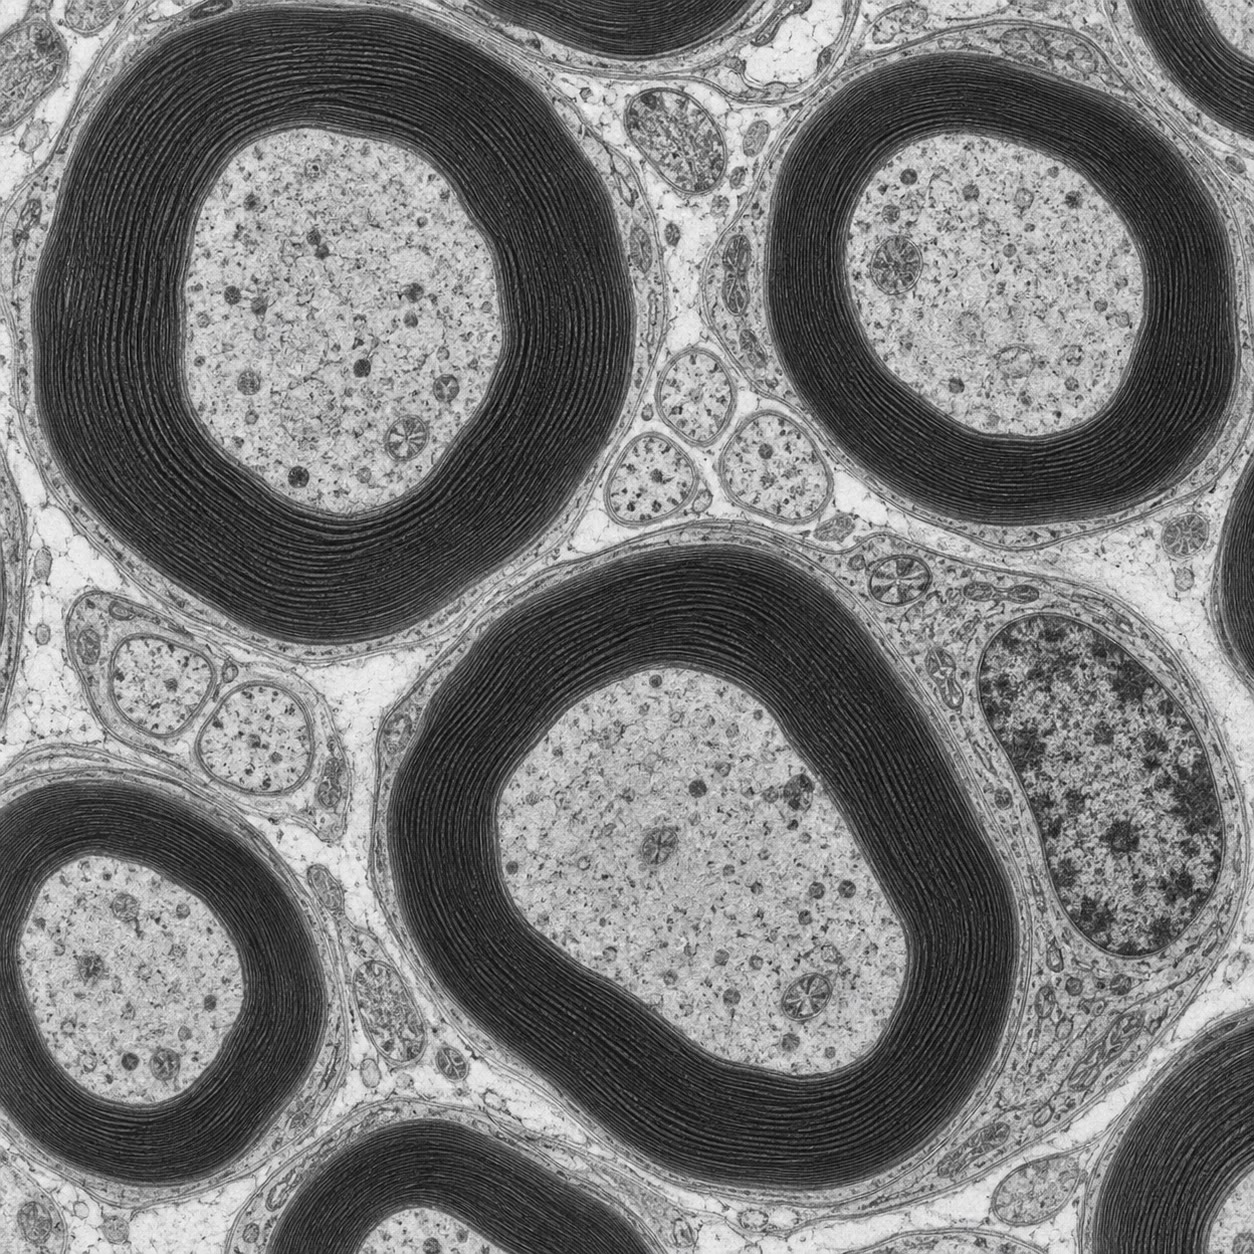
\includegraphics[width=0.4\linewidth]{images/book4/ai/b4-20-myelinated-axons-tem.jpg}

{\small Left: a pyramidal \omterm{def:b2:neurons-synapses:neuron}{neuron} filled with dye --- the cell body,
the spiny \omterm{def:b2:neurons-synapses:neuron}{dendrites} that receive, and the thin \omterm{def:b2:neurons-synapses:neuron}{axon} that leaves the
base. Right: \omterm{def:b2:neurons-synapses:neuron}{axons} in cross-section under the electron microscope,
each wrapped in the dark spiral of its \omterm{def:b2:neurons-synapses:neuron}{myelin} sheath.}
\end{omfigure}

\section{The resting potential}

\begin{theorem}[The Nernst potential]\label{thm:b2:neurons-synapses:nernst}
\index{Nernst potential}\index{equilibrium potential}
A membrane permeable to one ion of charge $z$ separating
concentrations $c_{\text{out}}$ and $c_{\text{in}}$ settles at the
\emph{\omterm{thm:b2:neurons-synapses:nernst}{equilibrium potential}} at which the electrical force on the
ion balances its diffusion:
\[
E = \frac{RT}{zF}\ln\frac{c_{\text{out}}}{c_{\text{in}}} \approx \frac{\qty{61.5}{mV}}{z}\log_{10}\frac{c_{\text{out}}}{c_{\text{in}}} \quad (\qty{37}{\celsius}).
\]
A \omterm{def:b2:neurons-synapses:neuron}{neuron} holds \qty{140}{mmol/L} of potassium inside against
\qty{5}{mmol/L} outside, and \qty{15}{mmol/L} of sodium inside
against \qty{145}{mmol/L} outside, gradients built by the
sodium--potassium pump at the cost of a third of the cell's ATP.
Hence $E_{\mathrm K} = 61.5\log_{10}(5/140) = \qty{-89}{mV}$ and
$E_{\mathrm{Na}} = 61.5\log_{10}(145/15) = \qty{+61}{mV}$: if the
membrane let only potassium through it would sit at
\qty{-89}{mV}, if only sodium at \qty{+61}{mV}.
\end{theorem}
\begin{proof}
At equilibrium the electrochemical potential of the ion is the same
on both sides: $RT\ln c_{\text{in}} + zFV_{\text{in}} = RT\ln
c_{\text{out}} + zFV_{\text{out}}$, so $V_{\text{in}} -
V_{\text{out}} = (RT/zF)\ln(c_{\text{out}}/c_{\text{in}})$. At
\qty{310}{K}, $RT/F = \qty{26.7}{mV}$ and $\ln 10 \times 26.7 =
\qty{61.5}{mV}$. (Derived in the Year 1 volume from the Boltzmann
distribution; restated here.)
\end{proof}

\begin{theorem}[The resting potential as a weighted mean]\label{thm:b2:neurons-synapses:chord}
\index{resting potential}\index{conductance (membrane)}
If the membrane conducts several ions, each with conductance $g_i$
(the ease with which it passes, set by the number of open channels),
the steady potential at which the currents cancel is
\[
V = \frac{\sum_i g_i E_i}{\sum_i g_i},
\]
a mean of the \omterm{thm:b2:neurons-synapses:nernst}{equilibrium potentials} weighted by the conductances.
At rest a \omterm{def:b2:neurons-synapses:neuron}{neuron}'s membrane is about twenty times more permeable
to potassium than to sodium, so $V \approx (20\times(-89) +
61)/21 = \qty{-82}{mV}$; with the chloride and the small leaks
counted, the \omterm{thm:b2:neurons-synapses:chord}{resting potential} is \qty{-70}{mV}. The membrane rests
near $E_{\mathrm K}$ because potassium channels are open; whatever
opens sodium channels drags it toward $E_{\mathrm{Na}}$ --- and that
is the whole principle of nerve signalling.
\end{theorem}
\begin{proof}
Each ion carries a current $I_i = g_i(V - E_i)$ (Ohm's law, with
the driving force measured from the ion's own equilibrium). At a
steady potential the total current is zero: $\sum_i g_i(V - E_i) =
0$, whence $V\sum g_i = \sum g_iE_i$. (The full treatment, in which
the permeabilities enter through the Goldman--Hodgkin--Katz
equation, gives the same weighting to first order.)
\end{proof}

\section{The action potential}

\begin{proposition}[The impulse]\label{prop:b2:neurons-synapses:ap}
\index{action potential}\index{voltage-gated channel}\index{threshold}\index{refractory period}
The \omterm{def:b2:neurons-synapses:neuron}{axon} membrane holds \emph{voltage-gated sodium channels}, shut
at rest and opened by depolarisation. If a stimulus raises the
potential from \qty{-70}{mV} past a \emph{threshold} near
\qty{-55}{mV}, enough of them open to let in more sodium than the
potassium leak can offset; the potential rises, more channels open,
and within a fraction of a millisecond the membrane is swept toward
$E_{\mathrm{Na}}$ --- a \emph{positive feedback} that is explosive
and all-or-none. It peaks near \qty{+40}{mV} because the sodium
channels \emph{inactivate} within a millisecond of opening and
because slower \emph{voltage-gated potassium channels} open and
drive the potential back toward $E_{\mathrm K}$, overshooting to an
\emph{undershoot} before the potassium channels close. The
\emph{\omterm{prop:b2:neurons-synapses:ap}{action potential}} lasts about a millisecond; for another
millisecond or two the inactivated sodium channels cannot reopen
(the \emph{\omterm{prop:b2:neurons-synapses:ap}{refractory period}}), which limits the firing rate to a
few hundred per second and forces the impulse to travel one way.
Because it is all-or-none, the impulse carries no information in its
size: the \omterm{def:b2:neurons-synapses:neuron}{neuron} codes intensity in its \emph{frequency}. Some
$10^{4}$ sodium ions enter and as many potassium ions leave per
impulse --- a negligible change in concentration, restored by the
pump at leisure.
\end{proposition}
\begin{proof}[Evidence]
Hodgkin and Huxley (1952), using the squid's giant \omterm{def:b2:neurons-synapses:neuron}{axon} (half a
millimetre thick, so that a wire could be threaded inside it) and a
feedback amplifier that held the membrane potential at any chosen
value (the \emph{voltage clamp}) while recording the current needed
to hold it, separated the current into an early inward component
that vanished when sodium was removed from the bath and a later
outward component carried by potassium; measured how each
conductance rose and fell with time at each voltage; and, fitting
each with a few equations, computed the \omterm{prop:b2:neurons-synapses:ap}{action potential}'s shape,
threshold, speed and \omterm{prop:b2:neurons-synapses:ap}{refractory period} from the two conductances
alone. Every prediction held. The channels themselves were seen
twenty-five years later, one at a time, with the patch clamp;
tetrodotoxin (the pufferfish poison) blocks the sodium channel
and abolishes the impulse, tetraethylammonium blocks the potassium
channel and prolongs it.
\end{proof}

\begin{omfigure}
\begin{tikzpicture}
\begin{axis}[
  width=0.9\linewidth, height=6.4cm,
  axis x line=bottom, axis y line=left,
  xmin=0, xmax=4, ymin=-100, ymax=60,
  xlabel={time (ms)}, ylabel={membrane potential (mV)},
  xlabel style={font=\small, at={(axis description cs:0.5,-0.1)}, anchor=north},
  ylabel style={font=\small},
  tick label style={font=\small}, xtick={0,1,2,3,4}, ytick={-90,-70,-55,0,40},
  legend style={font=\scriptsize, at={(0.97,0.95)}, anchor=north east, draw=none},
  clip=false,
]
\addplot[very thick, omDef] coordinates {(0,-70) (0.4,-70) (0.5,-64) (0.6,-55) (0.7,-30) (0.8,10) (0.9,35) (1.0,40) (1.1,30) (1.2,10) (1.35,-20) (1.5,-50) (1.7,-75) (1.9,-85) (2.2,-82) (2.6,-76) (3.2,-71) (4,-70)};
\addlegendentry{membrane potential}
\addplot[thick, omThm, dashed] coordinates {(0,0) (0.5,0) (0.6,5) (0.7,20) (0.8,35) (0.9,30) (1.0,20) (1.1,8) (1.2,3) (1.4,0) (4,0)};
\addlegendentry{$g_{\mathrm{Na}}$ (relative)}
\addplot[thick, omProp, dashed] coordinates {(0,0) (0.6,0) (0.8,2) (1.0,8) (1.2,16) (1.4,20) (1.7,17) (2.0,10) (2.4,4) (3.0,1) (4,0)};
\addlegendentry{$g_{\mathrm K}$ (relative)}
\draw[dashed, gray] (axis cs:0,-55) -- (axis cs:4,-55); \node[font=\scriptsize, anchor=south east] at (axis cs:4,-55) {threshold};
\draw[dashed, gray] (axis cs:0,-89) -- (axis cs:4,-89); \node[font=\scriptsize, anchor=south east] at (axis cs:3.7,-89) {$E_{\mathrm K}$};
\draw[<->, gray] (axis cs:1.0,50) -- (axis cs:2.5,50); \node[font=\scriptsize, anchor=south, gray] at (axis cs:1.75,50) {refractory};
\end{axis}
\end{tikzpicture}

{\small An \omterm{prop:b2:neurons-synapses:ap}{action potential}. Past threshold the sodium conductance
(red) rises explosively and drives the potential toward
$E_{\mathrm{Na}}$; it inactivates as the potassium conductance
(orange) rises and returns the membrane toward $E_{\mathrm K}$, with
an undershoot. Below the threshold line, nothing happens.}
\end{omfigure}

\section{Conduction}

\begin{theorem}[The cable and its length constant]\label{thm:b2:neurons-synapses:cable}
\index{length constant}\index{cable equation}\index{conduction velocity}
An \omterm{def:b2:neurons-synapses:neuron}{axon} is a leaky cable: current injected at a point flows along
the cytoplasm (resistance $r_i$ per unit length) and leaks out
through the membrane (resistance $r_m$ times unit length). A steady
depolarisation $V_0$ at $x = 0$ decays along the \omterm{def:b2:neurons-synapses:neuron}{axon} as
\[
V(x) = V_0\,e^{-x/\lambda}, \qquad \lambda = \sqrt{\frac{r_m}{r_i}} = \sqrt{\frac{R_m\,d}{4R_i}},
\]
where $d$ is the diameter and $R_m$, $R_i$ the membrane's and
cytoplasm's specific resistances. The \emph{\omterm{thm:b2:neurons-synapses:cable}{length constant}}
$\lambda$ is the distance over which a passive signal falls to a
third: about \qty{0.5}{mm} for a \qty{1}{\micro m} \omterm{def:b2:neurons-synapses:neuron}{axon}, growing
as the square root of the diameter. An \omterm{prop:b2:neurons-synapses:ap}{action potential} propagates
because the depolarisation at its front, spreading passively ahead
by about $\lambda$, brings the next stretch of membrane to
threshold, which regenerates it at full size; the further ahead
it reaches, the faster the wave, so the \omterm{thm:b2:neurons-synapses:cable}{conduction velocity} also
grows roughly as $\sqrt{d}$ --- from \qty{1}{m/s} in a thin
unmyelinated fibre to \qty{20}{m/s} in the squid's giant \omterm{def:b2:neurons-synapses:neuron}{axon}.
\end{theorem}
\begin{proof}
Let $i(x)$ be the axial current and $V(x)$ the membrane
depolarisation. Ohm's law along the axoplasm gives $\mathrm{d}V/
\mathrm{d}x = -r_i\,i$; conservation of charge, with the leak through
the membrane, gives $\mathrm{d}i/\mathrm{d}x = -V/r_m$. Combining,
$\mathrm{d}^{2}V/\mathrm{d}x^{2} = V/(r_m r_i)$, whose decaying
solution is $V_0 e^{-x/\lambda}$ with $\lambda^{2} = r_m/r_i$. For a
cylinder, $r_m = R_m/(\pi d)$ and $r_i = 4R_i/(\pi d^{2})$, so
$\lambda^{2} = R_m d/4R_i$. With $R_m = \qty{1}{\ohm.m^2}$, $R_i =
\qty{1}{\ohm.m}$ and $d = \qty{1}{\micro m}$: $\lambda = \sqrt{10^{-6}
/4} = \qty{0.5}{mm}$.
\end{proof}

\begin{proposition}[Myelin and saltatory conduction]\label{prop:b2:neurons-synapses:myelin}
\index{saltatory conduction}\index{node of Ranvier}
\omterm{def:b2:neurons-synapses:neuron}{Myelin} multiplies $r_m$ by the number of membrane turns and divides
the membrane's capacitance by the same factor, so that under the
sheath almost no current leaks and little charge is needed to
change the potential: the depolarisation spreads passively along an
internode of a millimetre with little loss, and the \omterm{prop:b2:neurons-synapses:ap}{action potential}
is regenerated only at the nodes, where the sodium channels are
concentrated. The impulse thus \emph{jumps} from node to node
(\emph{\omterm{prop:b2:neurons-synapses:myelin}{saltatory conduction}}), at \qty{100}{m/s} in a
\qty{20}{\micro m} fibre --- a speed an unmyelinated \omterm{def:b2:neurons-synapses:neuron}{axon} would need
to be centimetres thick to reach --- and at a fraction of the
metabolic cost, since sodium enters only at the nodes. \omterm{def:b2:neurons-synapses:neuron}{Myelin} is
the vertebrate invention that made a large, fast nervous system
possible in a small body; in multiple sclerosis the sheath is
destroyed patch by patch, the \omterm{thm:b2:neurons-synapses:cable}{length constant} collapses, and the
impulses fail.
\end{proposition}

\begin{omfigure}
\begin{tikzpicture}[every node/.style={font=\scriptsize}, >=stealth]
  % unmyelinated
  \begin{scope}
    \draw[thick, fill=omDef!10] (0,0) rectangle (11,0.5);
    \foreach \x in {0.5,1.0,...,10.5} \draw[omThm, ->] (\x,0.25) -- (\x,0.9);
    \node[anchor=east] at (-0.2,0.25) {unmyelinated};
    \node[anchor=west] at (11.2,0.25) {\qty{1}{m/s}};
    \node[above] at (5.5,1.0) {the impulse is regenerated at every point};
  \end{scope}
  % myelinated
  \begin{scope}[yshift=-2.4cm]
    \draw[thick, fill=omDef!10] (0,0) rectangle (11,0.5);
    \foreach \x in {0.3,2.5,4.7,6.9,9.1} \fill[omExo!60] (\x,-0.15) rectangle (\x+1.9,0.65);
    \foreach \x in {2.35,4.55,6.75,8.95} \draw[omThm, ->] (\x,0.25) -- (\x,0.9);
    \foreach \x in {2.35,4.55,6.75} \draw[->, thick, omThm, dashed] (\x+0.1,1.1) .. controls (\x+1.1,1.6) .. (\x+2.1,1.1);
    \node[anchor=east] at (-0.2,0.25) {myelinated};
    \node[anchor=west] at (11.2,0.25) {\qty{100}{m/s}};
    \node[below] at (1.25,-0.2) {myelin internode};
    \node[below] at (4.55,-0.2) {node of Ranvier};
    \node[above] at (5.5,1.6) {regenerated only at the nodes: saltatory};
  \end{scope}
\end{tikzpicture}

{\small Conduction with and without \omterm{def:b2:neurons-synapses:neuron}{myelin}. In a bare \omterm{def:b2:neurons-synapses:neuron}{axon} the
impulse is regenerated all along; under \omterm{def:b2:neurons-synapses:neuron}{myelin} the signal spreads
passively along each internode and is regenerated at the nodes, and
the impulse travels a hundred times faster.}
\end{omfigure}

\section{The synapse}

\begin{definition}[Chemical and electrical synapses]\label{def:b2:neurons-synapses:synapse}
\index{synapse}\index{neurotransmitter}\index{postsynaptic potential}
At a \emph{synapse} a \omterm{def:b2:neurons-synapses:neuron}{neuron}'s terminal meets a target --- another
\omterm{def:b2:neurons-synapses:neuron}{neuron}, a \omterm{def:b2:cell-differentiation:myogenesis}{muscle fibre}, a gland cell. In an \emph{electrical}
synapse gap junctions join the two cells and current passes directly
--- fast, bidirectional, without amplification, used where speed and
synchrony matter (escape reflexes, the \omterm{def:b2:heart:anatomy}{heart}). In a \emph{chemical}
synapse the cells are separated by a cleft of \qty{20}{nm} and the
signal is a molecule. An \omterm{prop:b2:neurons-synapses:ap}{action potential} arriving at the terminal
opens voltage-gated calcium channels; calcium enters and, within a
fraction of a millisecond, makes vesicles of \emph{neurotransmitter}
fuse with the membrane and empty into the cleft; the transmitter
diffuses across in microseconds and binds receptors on the
postsynaptic membrane --- either ion channels that it opens
(\emph{ionotropic}, fast) or \omterm{prop:b2:cell-signalling:gpcr}{G-protein-coupled receptors}
(\emph{metabotropic}, slower, \cref{ch:b2:cell-signalling}); the
resulting current shifts the postsynaptic potential by a few
millivolts, up (an \emph{excitatory postsynaptic potential}, from
channels passing sodium) or down (an \emph{inhibitory} one, from
channels passing chloride or potassium); and the transmitter is
removed within milliseconds by an enzyme or a transporter. The
delay is half a millisecond; the price buys one-way transmission,
amplification, inhibition, and modifiability --- everything a
nervous system needs beyond mere conduction.
\end{definition}

\begin{omfigure}
\begin{tikzpicture}[every node/.style={font=\scriptsize}, >=stealth]
  % presynaptic terminal
  \draw[thick, fill=omDef!10] (0,0) .. controls (0,2.6) and (3.6,2.6) .. (3.6,0.2) -- (3.6,-0.2) .. controls (3.6,-2.6) and (0,-2.6) .. (0,0);
  \draw[very thick, omDef] (-2.2,0) -- (0.1,0); \node[omDef, above] at (-1.1,0.05) {axon};
  \foreach \p in {(2.0,1.0),(2.6,0.5),(2.7,-0.4),(2.1,-1.0),(1.6,0.2)} \draw[thick, fill=omProp!40] \p circle (0.25);
  \draw[thick, fill=omProp!40] (3.3,0.1) arc (90:-90:0.25) -- cycle;
  \foreach \p in {(3.75,0.2),(3.85,-0.1),(3.7,-0.35),(3.9,0.4)} \fill[omProp] \p circle (0.05);
  \fill[omThm] (3.45,1.3) circle (0.06); \node[omThm, anchor=east] at (3.35,1.45) {Ca$^{2+}$ enters};
  \draw[->, omThm] (3.9,1.5) -- (3.55,1.35);
  % cleft
  \node[align=center, anchor=north] at (3.85,-2.75) {cleft\\\qty{20}{nm}};
  \draw[gray] (3.85,-2.7) -- (3.85,-1.2);
  % postsynaptic
  \draw[thick, fill=omExo!15] (4.1,-2.6) rectangle (8.2,2.6);
  \foreach \y in {0.9,0.3,-0.3,-0.9} \draw[thick, fill=omDef!40] (4.05,\y-0.15) rectangle (4.45,\y+0.15);
  \node[anchor=west, align=left] at (4.6,0.3) {receptors: channels\\open, ions flow,\\postsynaptic\\potential};
  \node[anchor=west, align=left] at (4.6,-1.7) {transmitter removed\\by enzyme or\\transporter};
  \node[anchor=west] at (4.6,2.2) {postsynaptic cell};
  % labels
  \node[align=center, anchor=north] at (1.8,-2.75) {vesicles of\\transmitter};
  \node[anchor=south] at (1.8,2.75) {presynaptic terminal};
\end{tikzpicture}

{\small A chemical \omterm{def:b2:neurons-synapses:synapse}{synapse}. The impulse admits calcium, vesicles
fuse and release transmitter into the cleft, receptors on the
target open channels, and the transmitter is cleared within
milliseconds.}
\end{omfigure}

\begin{theorem}[Quantal release]\label{thm:b2:neurons-synapses:quantal}
\index{quantal release}\index{miniature potential}
Transmitter is released in packets --- \emph{quanta}, one vesicle
each --- and the number $k$ released by one impulse is a random
variable. If the terminal holds $n$ release sites each releasing
with probability $p$, and $p$ is small, $k$ is approximately Poisson
with mean $m = np$:
\[
P(k) = \frac{m^{k}e^{-m}}{k!}, \qquad P(0) = e^{-m}, \qquad
m = \ln\frac{\text{number of trials}}{\text{number of failures}}.
\]
The mean quantal content $m$ can therefore be read from the
fraction of impulses that release nothing, and checked against the
mean response divided by the size of one quantum. At a
\omterm{prop:b2:neurons-synapses:integration}{neuromuscular junction} $m$ is a few hundred --- transmission never
fails; at a central \omterm{def:b2:neurons-synapses:synapse}{synapse} it is often near one, and the \omterm{def:b2:neurons-synapses:synapse}{synapse}
transmits on a fraction of the impulses.
\end{theorem}
\begin{proof}
With $n$ independent sites each releasing with probability $p$, $k$
is binomial; for large $n$ and small $p$ with $np = m$ fixed, the
binomial tends to the Poisson law (the mathematics series, Year 2).
$P(0) = e^{-m}$ gives $m$ from the failures. Katz's check is that
the same $m$, put into the Poisson formula, predicts the observed
fractions of responses of one, two and three quanta.
\end{proof}
\begin{proof}[Evidence]
Fatt and Katz (1952) recorded from a frog \omterm{def:b2:cell-differentiation:myogenesis}{muscle fibre} at rest
small spontaneous depolarisations of about \qty{0.5}{mV}, all the
same size, at random intervals --- the \emph{miniature end-plate
potentials}, each the effect of one vesicle. Lowering the calcium in
the bath reduced the response to nerve stimulation until it
fluctuated among 0, 1, 2 or 3 multiples of the miniature size;
the frequencies of the multiples followed the Poisson law with the
$m$ computed from the failures. Del Castillo and Katz thus showed
that release is quantal, that calcium controls the probability of
release and not the size of a quantum, and electron microscopy
showed the vesicles that are the quanta.
\end{proof}

\begin{proposition}[Integration: the neuron as a decision]\label{prop:b2:neurons-synapses:integration}
\index{summation}\index{axon hillock}\index{neuromuscular junction}
A central \omterm{def:b2:neurons-synapses:neuron}{neuron} receives thousands of \omterm{def:b2:neurons-synapses:synapse}{synapses}, excitatory and
inhibitory, on its \omterm{def:b2:neurons-synapses:neuron}{dendrites} and soma. Each \omterm{def:b2:neurons-synapses:synapse}{postsynaptic potential}
is small and decays passively, with the cable's \omterm{thm:b2:neurons-synapses:cable}{length constant} in
space and the membrane's time constant (a few milliseconds) in
time; they add --- \emph{spatial summation} of inputs arriving
together, \emph{temporal summation} of inputs arriving in quick
succession --- and the sum is read at the \emph{\omterm{prop:b2:neurons-synapses:integration}{axon hillock}}, where
the sodium channels are densest and the threshold lowest. If the
sum crosses threshold the \omterm{def:b2:neurons-synapses:neuron}{axon} fires, at a rate that rises with the
excess; inhibitory inputs subtract, and an inhibitory \omterm{def:b2:neurons-synapses:synapse}{synapse} close
to the hillock can veto a distant excitatory one. The
\omterm{prop:b2:neurons-synapses:integration}{neuromuscular junction} is the exception that shows the rule: one
motor terminal, releasing hundreds of quanta of acetylcholine onto
receptors that are also the channels, gives an end-plate potential
of \qty{50}{mV}, far above threshold --- every impulse in the motor
nerve produces a muscle \omterm{prop:b2:neurons-synapses:ap}{action potential}
(\cref{ch:b2:muscle-movement}). Curare, which blocks the receptor,
paralyses; nerve gases, which block the enzyme that removes
acetylcholine, paralyse by the opposite excess.
\end{proposition}

\begin{example}[Transmitters and drugs]\label{ex:b2:neurons-synapses:transmitters}
Acetylcholine at the \omterm{prop:b2:neurons-synapses:integration}{neuromuscular junction} and in the autonomic
system; glutamate, the main excitatory transmitter of the brain,
and GABA, the main inhibitory one; the monoamines noradrenaline,
dopamine and serotonin, which modulate whole circuits from a few
thousand cells; and dozens of peptides. Almost every drug that acts
on the mind acts on a \omterm{def:b2:neurons-synapses:synapse}{synapse}: benzodiazepines strengthen GABA's
channel, antidepressants block serotonin's transporter, cocaine
blocks dopamine's, opiates mimic a peptide, nicotine mimics
acetylcholine on one receptor and atropine blocks it on another,
botulinum toxin cuts the proteins that fuse the vesicle. The \omterm{def:b2:neurons-synapses:synapse}{synapse}
is where the chemistry of \cref{ch:b2:cell-signalling} and the
electricity of this chapter meet, and where a nervous system learns:
\omterm{def:b2:neurons-synapses:synapse}{synapses} that are used strengthen, and that strengthening (the
Year 3 volume) is memory.
\end{example}

\section{Exercises}

\begin{exercise}[$\star$]\label{exo:b2:neurons-synapses:1}
Name the parts of a \omterm{def:b2:neurons-synapses:neuron}{neuron} and the function of each, and say what
\omterm{def:b2:neurons-synapses:neuron}{myelin} is made of and what it does.
\end{exercise}

\begin{exercise}[$\star$]\label{exo:b2:neurons-synapses:2}
Describe the phases of an \omterm{prop:b2:neurons-synapses:ap}{action potential} and the channel events
that cause each. Why is it all-or-none, and why does it not travel
backwards?
\end{exercise}

\begin{exercise}[$\star$]\label{exo:b2:neurons-synapses:3}
List the steps of transmission at a chemical \omterm{def:b2:neurons-synapses:synapse}{synapse} from the
arrival of the impulse to the removal of the transmitter.
\end{exercise}

\begin{exercise}[$\star$]\label{exo:b2:neurons-synapses:4}
Compare electrical and chemical \omterm{def:b2:neurons-synapses:synapse}{synapses} in speed, direction,
amplification and the possibility of inhibition.
\end{exercise}

\begin{exercise}[$\star\star$]\label{exo:b2:neurons-synapses:5}
Compute the \omterm{thm:b2:neurons-synapses:nernst}{Nernst potentials} at \qty{37}{\celsius} for potassium
(140 in, 5 out), sodium (15 in, 145 out), chloride (10 in, 110 out)
and calcium (\qty{1e-4}{} in, 2 out, in \unit{mmol/L}). Which way
does each ion flow when the membrane is at \qty{-70}{mV}?
\end{exercise}

\begin{exercise}[$\star\star$]\label{exo:b2:neurons-synapses:6}
With $E_{\mathrm K} = \qty{-89}{mV}$ and $E_{\mathrm{Na}} =
\qty{+61}{mV}$, compute the membrane potential when $g_{\mathrm K} :
g_{\mathrm{Na}} = 20 : 1$ (rest), $1 : 20$ (the peak of the impulse)
and $50 : 1$ (the undershoot). Explain each state.
\end{exercise}

\begin{exercise}[$\star\star$]\label{exo:b2:neurons-synapses:7}
\omterm{thm:b2:neurons-synapses:cable}{Conduction velocity} scales as $\sqrt d$ in unmyelinated \omterm{def:b2:neurons-synapses:neuron}{axons}, with
\qty{1}{m/s} at \qty{1}{\micro m}. Compute the velocity of a
\qty{0.5}{mm} squid \omterm{def:b2:neurons-synapses:neuron}{axon}. A myelinated \qty{20}{\micro m} fibre
conducts at \qty{100}{m/s}: how thick would an unmyelinated \omterm{def:b2:neurons-synapses:neuron}{axon} have
to be to match it? How long does an impulse take from the spinal
cord to the toe (\qty{1}{m}) in each fibre?
\end{exercise}

\begin{exercise}[$\star\star$]\label{exo:b2:neurons-synapses:8}
In 200 stimulations of a \omterm{def:b2:neurons-synapses:synapse}{synapse} in low calcium, 74 produce no
response. Compute the mean quantal content and the predicted
fractions of responses of one, two and three quanta. The single
quantum is \qty{0.5}{mV}: what mean response is expected?
\end{exercise}

\begin{exercise}[$\star\star$]\label{exo:b2:neurons-synapses:9}
A \omterm{def:b2:neurons-synapses:neuron}{neuron}'s \omterm{prop:b2:neurons-synapses:ap}{refractory period} is \qty{2}{ms}. What is its maximal
firing rate? A sensory \omterm{def:b2:neurons-synapses:neuron}{neuron} fires at 20 impulses a second for a
light touch and 200 for a hard one: what is coded, and by what?
\end{exercise}

\begin{exercise}[$\star\star\star$]\label{exo:b2:neurons-synapses:10}
Compute the \omterm{thm:b2:neurons-synapses:cable}{length constant} for $R_m = \qty{1}{\ohm.m^2}$, $R_i =
\qty{1}{\ohm.m}$ and diameters of 1, 10 and \qty{500}{\micro m}. \omterm{def:b2:neurons-synapses:neuron}{Myelin}
multiplies $R_m$ by 200: recompute for \qty{10}{\micro m}. Explain
why an internode of \qty{1}{mm} works and why a demyelinated stretch
of \qty{3}{mm} blocks the impulse.
\end{exercise}

\begin{exercise}[$\star\star\star$]\label{exo:b2:neurons-synapses:11}
Predict the effect on the \omterm{prop:b2:neurons-synapses:ap}{action potential} and on transmission at
the \omterm{prop:b2:neurons-synapses:integration}{neuromuscular junction} of: tetrodotoxin; tetraethylammonium; a
bath without calcium; curare; an acetylcholinesterase inhibitor;
botulinum toxin.
\end{exercise}

\begin{exercise}[$\star\star\star$]\label{exo:b2:neurons-synapses:12}
``A chemical \omterm{def:b2:neurons-synapses:synapse}{synapse} costs half a millisecond and buys a nervous
system.'' Discuss what the delay pays for --- one-way transmission,
amplification, inhibition, plasticity --- and where the body uses
electrical \omterm{def:b2:neurons-synapses:synapse}{synapses} instead.
\end{exercise}

\section{Problem: The Knee Jerk Timed}

\begin{problem}[{Weekend problem --- the stretch reflex followed from
the tendon tap to the kick, with the neuron's resting potential
computed, the impulse's conduction timed along the two limbs of the
arc, the synapse's quantal content measured, and the whole latency
accounted for, ending on the resting potential, the conduction times,
the quantal content and the reflex latency}]
\label{pb:b2:neurons-synapses:1}
Data at \qty{37}{\celsius}: potassium 140 in, 4 out; sodium 12 in,
145 out (\unit{mmol/L}); $g_{\mathrm K} : g_{\mathrm{Na}} = 25 : 1$
at rest. Sensory and motor \omterm{def:b2:neurons-synapses:neuron}{axons}: \qty{15}{\micro m}, myelinated,
\qty{90}{m/s}, \qty{0.9}{m} each way. Synaptic delay \qty{0.6}{ms};
muscle activation after its own \omterm{prop:b2:neurons-synapses:ap}{action potential} \qty{5}{ms}.
Central \omterm{def:b2:neurons-synapses:synapse}{synapse} in low calcium: 300 trials, 111 failures. Quantum
\qty{0.4}{mV}; threshold \qty{15}{mV} above rest. $R_m =
\qty{1}{\ohm.m^2}$, $R_i = \qty{1}{\ohm.m}$; \omterm{def:b2:neurons-synapses:neuron}{myelin} multiplies $R_m$
by 250.

\medskip
\noindent\textbf{Part I --- The resting \omterm{def:b2:neurons-synapses:neuron}{neuron}.}
\begin{enumerate}
  \item Compute $E_{\mathrm K}$ and $E_{\mathrm{Na}}$.
  \item Compute the \omterm{thm:b2:neurons-synapses:chord}{resting potential} from the conductance ratio.
  \item The extracellular potassium rises to \qty{8}{mmol/L} (as
        after intense exercise). Recompute $E_{\mathrm K}$ and the
        \omterm{thm:b2:neurons-synapses:chord}{resting potential}, and say what this does to excitability.
  \item The pump stops. Explain what happens to the gradients and the
        potential over hours, and why the cell swells.
  \item How many sodium ions enter a \qty{15}{\micro m} \omterm{def:b2:neurons-synapses:neuron}{axon} per
        millimetre per impulse if the membrane's capacitance is
        \qty{0.01}{F/m^2} and the potential swings by \qty{100}{mV}?
        ($Q = CV$; one ion carries \qty{1.6e-19}{C}.)
  \item By what fraction does that change the internal sodium
        concentration (\omterm{def:b2:neurons-synapses:neuron}{axon} volume per millimetre)?
  \item The pump exports three sodium ions per ATP. How many ATP
        does it cost to undo one impulse per millimetre of \omterm{def:b2:neurons-synapses:neuron}{axon}?
\end{enumerate}

\medskip
\noindent\textbf{Part II --- Conduction.}
\begin{enumerate}[resume]
  \item Compute the time for the sensory impulse to reach the spinal
        cord and for the motor impulse to reach the muscle.
  \item Compute the \omterm{thm:b2:neurons-synapses:cable}{length constant} of a bare \qty{15}{\micro m}
        \omterm{def:b2:neurons-synapses:neuron}{axon} and of the same \omterm{def:b2:neurons-synapses:neuron}{axon} under \omterm{def:b2:neurons-synapses:neuron}{myelin}.
  \item An internode is \qty{1.5}{mm}. What fraction of the nodal
        depolarisation reaches the next node passively, with and
        without \omterm{def:b2:neurons-synapses:neuron}{myelin}? Which case can bring the next node to
        threshold (\qty{15}{mV} from a \qty{100}{mV} impulse)?
  \item Unmyelinated, the same \omterm{def:b2:neurons-synapses:neuron}{axon} would conduct at $\sqrt{15}$
        m/s. Compute the round trip and comment.
  \item A patch of \qty{4}{mm} loses its \omterm{def:b2:neurons-synapses:neuron}{myelin}. Compute the
        fraction of the signal crossing it and say whether the reflex
        survives.
  \item Why does the \omterm{prop:b2:neurons-synapses:ap}{refractory period} make the impulse travel in
        one direction only along the sensory \omterm{def:b2:neurons-synapses:neuron}{axon}?
\end{enumerate}

\medskip
\noindent\textbf{Part III --- The \omterm{def:b2:neurons-synapses:synapse}{synapse}.}
\begin{enumerate}[resume]
  \item Compute the mean quantal content $m$ from the failures.
  \item Compute the predicted fractions of responses of 1, 2 and 3
        quanta, and the expected numbers among the 300 trials.
  \item Compute the mean \omterm{def:b2:neurons-synapses:synapse}{postsynaptic potential}.
  \item In normal calcium the same \omterm{def:b2:neurons-synapses:synapse}{synapse} has $m = 60$. What is the
        probability of a failure, and the mean response? Does one
        such \omterm{def:b2:neurons-synapses:synapse}{synapse} fire the motor \omterm{def:b2:neurons-synapses:neuron}{neuron}?
  \item The motor \omterm{def:b2:neurons-synapses:neuron}{neuron} receives \num{20} such sensory \omterm{def:b2:neurons-synapses:synapse}{synapses}
        active at once. Explain how they sum and whether threshold is
        reached.
  \item An inhibitory \omterm{def:b2:neurons-synapses:synapse}{synapse} on the same \omterm{def:b2:neurons-synapses:neuron}{neuron} opens chloride
        channels ($E_{\mathrm{Cl}} = \qty{-70}{mV}$, the \omterm{thm:b2:neurons-synapses:chord}{resting
        potential}). Explain how it can reduce the excitatory
        response without hyperpolarising the cell.
\end{enumerate}

\medskip
\noindent\textbf{Part IV --- The whole reflex.}
\begin{enumerate}[resume]
  \item Add up: sensory conduction, synaptic delay, motor conduction,
        neuromuscular delay (\qty{0.6}{ms}), muscle activation. Compare
        with the measured \qty{30}{ms}.
  \item Where does the rest of the measured latency come from?
  \item The reflex has one \omterm{def:b2:neurons-synapses:synapse}{synapse} (monosynaptic). Explain why a
        withdrawal reflex, with two or three \omterm{def:b2:neurons-synapses:synapse}{synapses} in the cord,
        is slower but more flexible.
  \item The same tap in a patient with peripheral demyelination
        gives a reflex \qty{60}{ms} late. Estimate the \omterm{thm:b2:neurons-synapses:cable}{conduction
        velocity} in her nerves.
  \item A dose of tetrodotoxin blocks half the sodium channels.
        Predict the effect on the threshold, the impulse and the
        reflex.
  \item State the result: the \omterm{thm:b2:neurons-synapses:chord}{resting potential}, the sensory and
        motor conduction times, the quantal content $m$, and the
        computed reflex latency.
\end{enumerate}
\end{problem}
